\documentclass[11pt]{article}
\usepackage[margin=1in]{geometry}
\usepackage{amsmath,amssymb,amsthm}
\usepackage{booktabs}
\usepackage{graphicx}
\usepackage{hyperref}
\usepackage{float}

\newcommand{\E}{\mathbb{E}}
\newcommand{\Var}{\operatorname{Var}}
\newcommand{\R}{\mathbb{R}}
\newcommand{\softplus}{\operatorname{softplus}}

\title{Data 37711 Homework 2 --- Problem 1\\
\large Heteroscedastic regression: modelling $\E[Y\mid X]$ and $\sqrt{\Var(Y\mid X)}$}
\author{Yiwen Chen}
\date{}

\begin{document}
\maketitle

Throughout, $f_\mu(x)\approx\E[Y\mid X=x]$ and $f_\sigma(x)\approx\sqrt{\Var(Y\mid X=x)}$.
The code is in \texttt{problem1.py}.

%==========================================================================
\section*{(a) Link function}

Write the network output as $g(x)=(g_1(x),g_2(x))\in\R^2$. The two outputs have different
constraints:
\begin{itemize}
  \item $f_\mu(x)$ is a mean and can be any real number, so we use the \textbf{identity link}
  \[
     f_\mu(x) = g_1(x).
  \]
  (Trip durations are positive, so $\exp$ or $\softplus$ could be used here as well, but the
  conditional mean is far from $0$ for nearly all trips, so the identity link is simplest.)
  \item $f_\sigma(x)$ is a standard deviation and must be strictly positive. We use the
  \textbf{softplus link} plus a small floor $\varepsilon>0$:
  \[
     f_\sigma(x) = \softplus(g_2(x)) + \varepsilon = \log\bigl(1+e^{g_2(x)}\bigr) + \varepsilon .
  \]
\end{itemize}
$\softplus:\R\to(0,\infty)$ is smooth, monotone, and grows only linearly for large inputs, so the
gradients do not blow up the way they can with $f_\sigma=\exp(g_2)$. The floor $\varepsilon$ stops
$f_\sigma$ from going to $0$, which would make the loss below go to $-\infty$ if the model fit a
single point exactly. An equally valid option is the exponential link
$f_\sigma(x)=\exp(g_2(x))$, which says the network predicts $\log\sigma$.

%==========================================================================
\section*{(b) Loss function}

Under the model $Y_i\mid X_i \sim \mathcal N\bigl(f_\mu(X_i),\, f_\sigma(X_i)^2\bigr)$, independently
over $i$, the conditional density of one observation is
\[
  p(y_i\mid x_i) = \frac{1}{\sqrt{2\pi}\,f_\sigma(x_i)}
     \exp\!\left(-\frac{(y_i-f_\mu(x_i))^2}{2 f_\sigma(x_i)^2}\right).
\]
The log-likelihood of the sample is
\[
  \log \prod_{i=1}^n p(y_i\mid x_i)
   = \sum_{i=1}^n\left[-\tfrac12\log(2\pi) - \log f_\sigma(x_i)
     - \frac{(y_i-f_\mu(x_i))^2}{2 f_\sigma(x_i)^2}\right].
\]
Maximizing the likelihood is the same as minimizing the average \textbf{Gaussian negative
log-likelihood}:
\begin{equation}\label{eq:nll}
  \boxed{\;
  \mathcal L(\theta) = \frac1n\sum_{i=1}^n\left[\log f_\sigma(x_i)
      + \frac{\bigl(y_i-f_\mu(x_i)\bigr)^2}{2 f_\sigma(x_i)^2}\right] + \tfrac12\log(2\pi)
  \;}
\end{equation}
where $\theta$ are the network weights and the constant does not affect the optimum.

\paragraph{Interpretation.} The squared error term is weighted by $1/f_\sigma^2$, so points the
model considers noisy count less when fitting the mean. The $\log f_\sigma$ term penalizes
predicting a large $\sigma$ everywhere. For a fixed $x$, minimizing the per-point loss over
$s=f_\sigma(x)$ gives
\[
 \frac{\partial}{\partial s}\Bigl[\log s + \frac{r^2}{2s^2}\Bigr]
   = \frac1s - \frac{r^2}{s^3} = 0 \;\Longrightarrow\; s^2 = r^2,
 \qquad r = y-f_\mu(x).
\]
Averaged over the noise in $Y\mid X=x$, the population minimizer is
$f_\sigma(x)^2 = \E[(Y-f_\mu(x))^2\mid X=x]$. Together with $f_\mu(x)=\E[Y\mid X=x]$ (from setting
$\partial/\partial f_\mu=0$), this is exactly the conditional variance. So \eqref{eq:nll}
estimates both target quantities. If $f_\sigma\equiv\sigma$ is a constant, \eqref{eq:nll} reduces to
the usual MSE loss for $f_\mu$ (up to scale), so this loss generalizes least squares.

%==========================================================================
\section*{(c) Fitting an MLP on the taxi data}

\paragraph{Data and split.}
\texttt{taxi\_trips.parquet} has $n=523{,}554$ trips, 7 standardized features and the target
\texttt{trip\_duration} (minutes). The target is right-skewed: median $8.6$, mean $10.4$, standard
deviation $7.75$, 99th percentile $37.1$, max $228$ minutes. I split the data at random into
70\% training (366{,}487), 15\% validation (78{,}533) and 15\% test (78{,}534) using a fixed seed. The
validation set is used only for early stopping and learning-rate scheduling. The test set is used
once, for the final numbers.

\paragraph{Model.}
An MLP $g:\R^7\to\R^2$ with hidden layers $(256,256,128)$ and SiLU activations, followed by the links
from (a) with $\varepsilon=10^{-3}$. For stable optimization I train on the standardized target
$\tilde y=(y-\bar y)/s_y$ (training mean and standard deviation) and map back with
$f_\mu = \bar y + s_y\tilde f_\mu$ and $f_\sigma = s_y\tilde f_\sigma$. The bias of the $\sigma$
output is initialized so that $\tilde f_\sigma\approx1$ at the start of training. The loss is
\eqref{eq:nll}, optimized with Adam (learning rate $10^{-3}$, batch size 1024). The learning rate is
halved when the validation NLL stops improving for 2 epochs. Training stops early after 6 epochs
without improvement, and the weights with the best validation NLL are restored.

\paragraph{Baselines.} Each baseline is also a Gaussian model $(\mu(x),\sigma(x))$, so all models
are scored with the same metrics:
\begin{enumerate}
 \item \textbf{Constant}: $\mu=\bar y_{\text{train}}$, $\sigma=s_{y,\text{train}}$ (ignores $x$).
 \item \textbf{Linear + constant $\sigma$}: OLS for the mean; $\sigma$ is the standard deviation of
 the training residuals.
 \item \textbf{Homoscedastic MLP}: the same architecture and training procedure for the mean,
 with one learned global $\sigma$. This baseline isolates the gain from modelling $\sigma(x)$.
\end{enumerate}

\paragraph{Results (test set).}
\begin{table}[H]\centering
\begin{tabular}{lcccccc}
\toprule
Model & RMSE & MAE & Gaussian NLL & \multicolumn{3}{c}{Coverage of central PI} \\
      & (min) & (min) & (nats) & 50\% & 90\% & 95\% \\
\midrule
Constant                    & 7.746 & 5.699 & 3.466 & 0.523 & 0.941 & 0.958 \\
Linear + const.\ $\sigma$   & 7.551 & 5.592 & 3.441 & 0.536 & 0.935 & 0.956 \\
Homoscedastic MLP           & \textbf{3.637} & \textbf{2.303} & 2.711 & 0.672 & 0.932 & 0.953 \\
Heteroscedastic MLP (ours)  & 3.754 & 2.368 & \textbf{2.648} & 0.602 & 0.938 & 0.961 \\
\bottomrule
\end{tabular}
\caption{Test-set results ($n=78{,}534$). NLL is $-\frac1n\sum\log\mathcal N(y_i;f_\mu,f_\sigma^2)$ in
minutes (lower is better). Coverage is the fraction of $y_i$ inside
$f_\mu\pm z_{\alpha}f_\sigma$; a calibrated model gets the nominal level.}
\end{table}

\begin{itemize}
\item \textbf{The MLPs beat both simple baselines by a wide margin.} RMSE drops from about 7.6 to
about 3.7 minutes. The linear model barely improves on the constant, because trip duration depends
mostly on the \emph{distance} between pickup and dropoff (roughly
$\lVert(\text{pickup})-(\text{dropoff})\rVert$), and a linear function of the coordinates cannot
represent that.
\item \textbf{Modelling $\sigma(x)$ improves the likelihood.} The heteroscedastic MLP has the best
test NLL (2.648 vs.\ 2.711 for the same network with one global $\sigma$). This is the model's
training objective and the right score for a probabilistic regressor. Figure~\ref{fig:sigma}
(left) shows that the predicted $\sigma$ tracks the realized error: when the test points are
binned by $f_\sigma(x)$, the RMSE in each bin is close to the predicted $\sigma$. The right panel
shows that the noise grows with the expected duration, from about 2 minutes for short trips to
about 15--20 minutes for hour-long trips. A single global $\sigma$ cannot capture this.
\item \textbf{The heteroscedastic MLP has slightly worse RMSE.} This trade-off is expected: the
loss \eqref{eq:nll} down-weights residuals at points with large $f_\sigma$, so the mean is fit
less aggressively where the data are noisy. Its training curve
(Figure~\ref{fig:curves}) also shows more overfitting (train NLL $0.46$ vs.\ val $0.57$ in
standardized units), so stronger regularization (weight decay or dropout) would probably help.
\item \textbf{The Gaussian assumption is only approximate.} Trip durations are right-skewed and
heavy-tailed. Even the heteroscedastic model over-covers at the 50\% level ($0.60$) and is close
to nominal at 90--95\%. In other words, the residuals have a sharper peak and heavier tails than a
Gaussian. A Gaussian on $\log Y$, or a Student-$t$ likelihood, would fit better, but we keep the
normal model as the problem specifies.
\end{itemize}

\begin{figure}[H]\centering
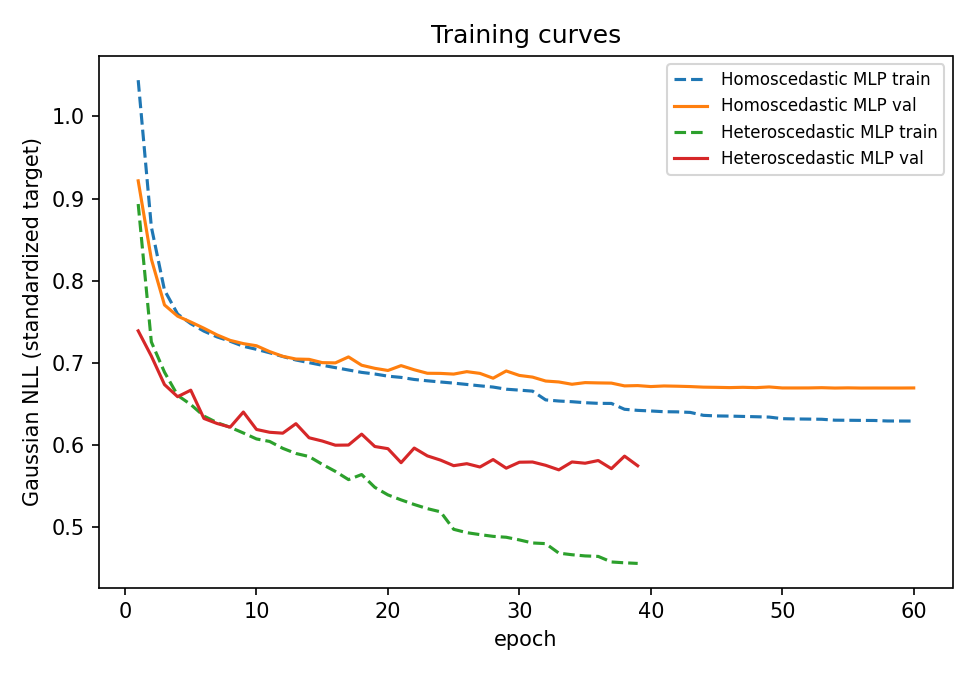
\includegraphics[width=0.62\textwidth]{problem1_training_curves.png}
\caption{Training and validation NLL (standardized target) for the two MLPs.}
\label{fig:curves}
\end{figure}
\begin{figure}[H]\centering
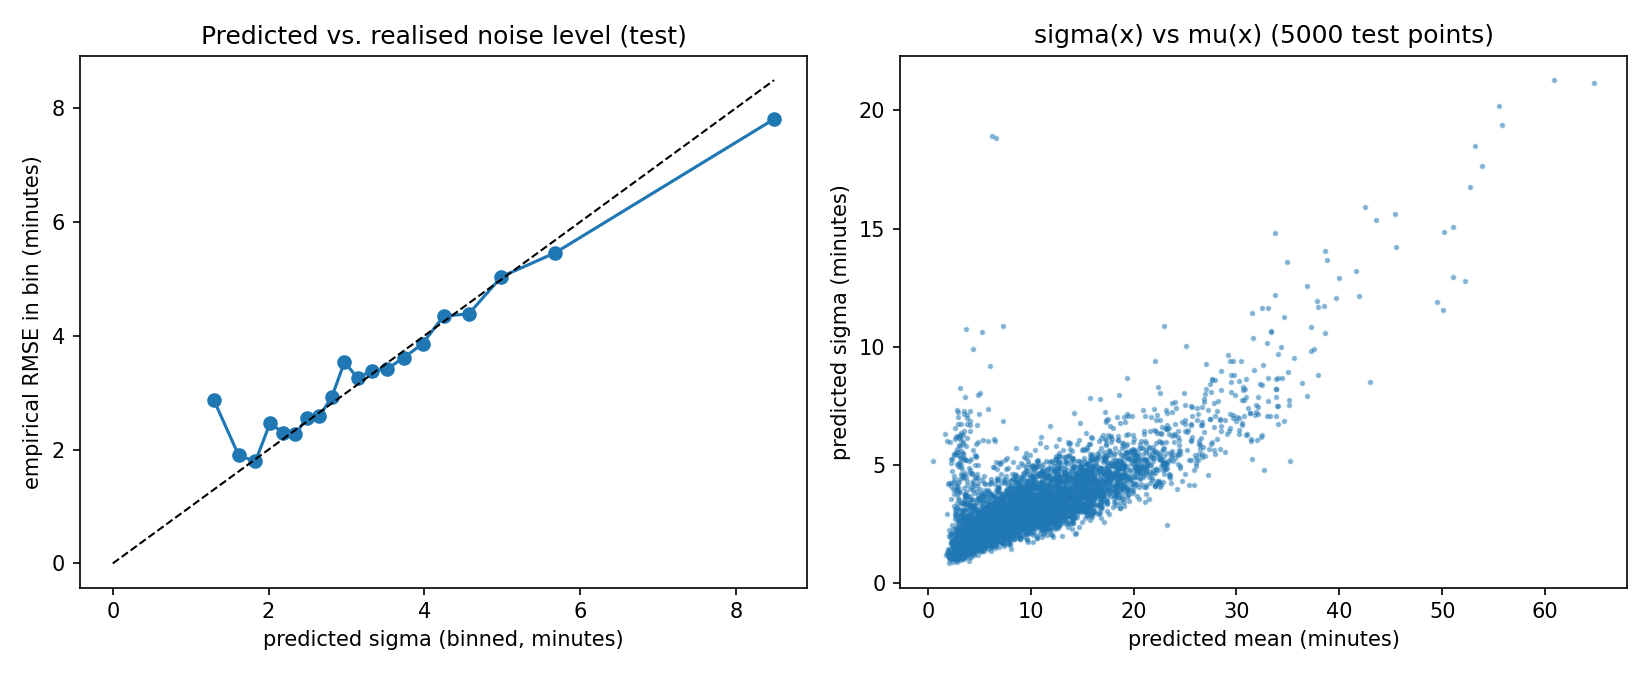
\includegraphics[width=\textwidth]{problem1_sigma.png}
\caption{Left: test points binned by predicted $f_\sigma(x)$; empirical RMSE in each bin vs.\ mean
predicted $\sigma$ (dashed line = perfect). Right: $f_\sigma(x)$ against $f_\mu(x)$.}
\label{fig:sigma}
\end{figure}


%==========================================================================
\section*{(d) Predicting $P(\text{trip} < 45\text{ min})$}

The fitted model gives a full predictive distribution
$Y\mid X=x\sim\mathcal N\bigl(f_\mu(x), f_\sigma(x)^2\bigr)$. Therefore
\[
 \boxed{\;
 \hat p(x) = P(Y<45\mid X=x)
   = P\!\left(\frac{Y-f_\mu(x)}{f_\sigma(x)} < \frac{45-f_\mu(x)}{f_\sigma(x)}\right)
   = \Phi\!\left(\frac{45-f_\mu(x)}{f_\sigma(x)}\right)\;}
\]
where $\Phi$ is the standard normal CDF. This uses both outputs. Two trips with the same predicted
mean of 30 minutes get different probabilities: a trip with $f_\sigma=5$ gets
$\Phi(3)\approx0.999$, and a trip with $f_\sigma=15$ gets $\Phi(1)\approx0.84$. A mean-only model
cannot tell these two cases apart. To classify, predict ``$<45$'' when $\hat p(x)\ge 0.5$. Because
$\Phi(0)=0.5$, this is equivalent to $f_\mu(x)\le45$: the 0.5-threshold decision depends only on
the mean, while the probability itself depends on both $f_\mu$ and $f_\sigma$.

%==========================================================================
\section*{(e) Evaluation of the probabilities on the test set}

For each test trip, the label is $z_i=\mathbf 1\{y_i<45\}$ and the prediction is
$\hat p_i=\Phi\bigl((45-f_\mu(x_i))/f_\sigma(x_i)\bigr)$. I report two proper scoring rules,
\[
 \text{Brier}=\frac1n\sum_i(\hat p_i-z_i)^2,\qquad
 \text{Log-loss}=-\frac1n\sum_i\bigl[z_i\log\hat p_i+(1-z_i)\log(1-\hat p_i)\bigr],
\]
plus the accuracy of $\mathbf 1\{\hat p_i\ge0.5\}$ and the AUC. A natural extra baseline is the
\emph{majority-class predictor}, which always outputs the training frequency
$\hat p=\hat P(Y<45)$.

\begin{table}[H]\centering
\begin{tabular}{lcccc}
\toprule
Model & Brier $\downarrow$ & Log-loss $\downarrow$ & Accuracy@0.5 $\uparrow$ & AUC $\uparrow$\\
\midrule
Majority class (train freq.\ $0.9956$) & 0.00444 & 0.02857 & 0.99554 & 0.500 \\
Constant Gaussian                      & 0.00446 & 0.05525 & 0.99554 & 0.500 \\
Linear + const.\ $\sigma$              & 0.00446 & 0.04662 & 0.99554 & 0.843 \\
Homoscedastic MLP                      & \textbf{0.00288} & 0.03170 & \textbf{0.99665} & 0.952 \\
Heteroscedastic MLP (ours)             & 0.00291 & \textbf{0.02063} & 0.99660 & \textbf{0.959} \\
\bottomrule
\end{tabular}
\caption{Test-set evaluation of $\hat p(x)=P(Y<45\mid x)$. 99.55\% of test trips (all but 350 of
78{,}534) are shorter than 45 minutes.}
\end{table}

\paragraph{Discussion.}
\begin{itemize}
\item \textbf{The classes are very imbalanced.} Only 350 of the 78{,}534 test trips (0.45\%) take 45
minutes or longer. A predictor that always says ``$<45$'' already reaches 99.55\% accuracy, so
accuracy on its own says little. The heteroscedastic MLP reaches 99.66\% accuracy, which removes
about 25\% of the majority-class errors. At the 0.5 threshold it flags 161 trips as long, and 122
of them really are long. The constant and linear baselines never predict a long trip.
\item \textbf{Proper scoring rules.} Both MLPs reduce the Brier score by about 35\% relative to the
baselines (0.0029 vs.\ 0.0044). On log-loss the heteroscedastic model is clearly best
(0.0206). It is the only model that beats the trivial majority-class predictor (0.0286), and it
improves on the homoscedastic MLP by 35\%. The homoscedastic MLP is \emph{worse} than the trivial
predictor on log-loss even though its Brier score and accuracy are good. The reason is that with
one global $\sigma\approx3.6$ minutes, a trip predicted at $\mu=25$ gets
$P(Y\ge45)=1-\Phi(5.5)\approx2\times10^{-8}$. When such a trip does take more than 45 minutes,
the log-loss charges about $\log(1/(2\times10^{-8}))\approx18$ nats. The heteroscedastic model
assigns larger $\sigma$ to long and uncertain trips, so it spreads probability into the tail
much more realistically. This is exactly where modelling $\sigma(x)$ matters.
\item \textbf{Calibration.} Figure~\ref{fig:rel} shows that all Gaussian models are
\emph{over-confident} at small predicted probabilities. Trips assigned $P(Y\ge45)<10^{-3}$ actually
take $\ge45$ minutes about $10^{-3}$--$10^{-2}$ of the time, because the right tail of trip
durations is heavier than a Gaussian tail. The heteroscedastic model is the closest to the
diagonal, and above about $0.05$ it is well calibrated. A heavier-tailed or log-scale likelihood
would reduce the remaining miscalibration.
\item As shown in (d), the 0.5-threshold decision is $f_\mu(x)\le45$, so it depends only on the
mean. That is why the two MLPs have nearly identical accuracy. The difference between them shows
up in the probabilities, which is what the Brier score, log-loss and calibration measure.
\end{itemize}

\begin{figure}[H]\centering
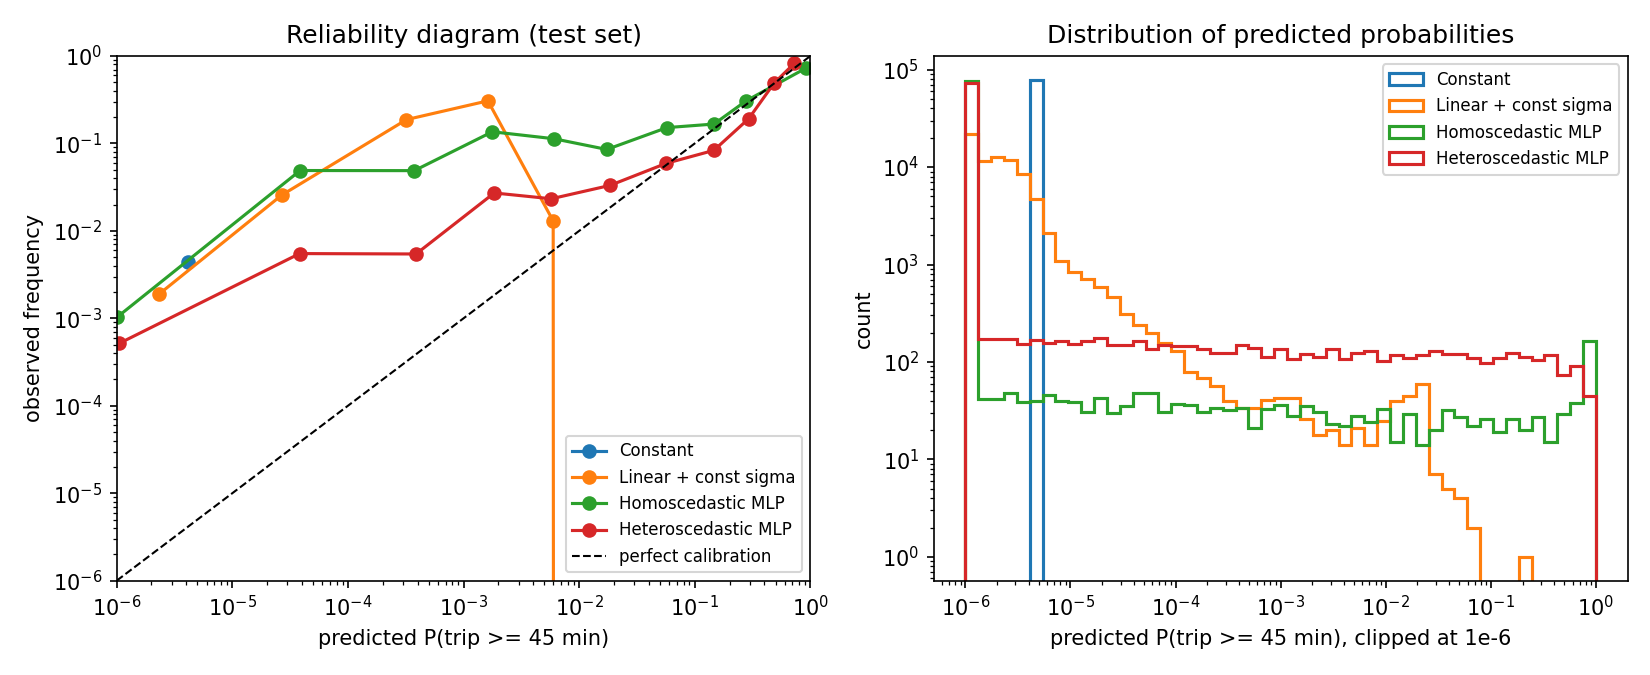
\includegraphics[width=\textwidth]{problem1_reliability.png}
\caption{Left: reliability diagram for the rare event $\{Y\ge45\}$ on the test set (log--log
axes; dashed line = perfect calibration). Right: histogram of predicted $P(Y\ge45)$, clipped at
$10^{-6}$.}
\label{fig:rel}
\end{figure}


\end{document}
